\let\negmedspace\undefined
\let\negthickspace\undefined
\documentclass[journal,12pt,onecolumn]{IEEEtran}
\usepackage{cite}
\usepackage{amsmath,amssymb,amsfonts,amsthm}
\usepackage{algorithmic}
\usepackage{amsmath}
\usepackage{graphicx}
\graphicspath{{./figs/}}
\usepackage{textcomp}
\usepackage{framed} 

\usepackage[utf8]{inputenc}
\usepackage{xcolor}
\usepackage{txfonts}
\usepackage{romannum}
\usepackage{listings}
\usepackage{enumitem}
\usepackage{mathtools}
\usepackage{gensymb}
\usepackage{comment}
\usepackage{caption}
\usepackage[breaklinks=true]{hyperref}
\usepackage{tkz-euclide} 
\usepackage{listings}
\usepackage{gvv}                                        
\usepackage{color}        
\usepackage[utf8]{inputenc}                                     
\usepackage{array}                                            
\usepackage{longtable}         
\usepackage{multicol}                              
\usepackage{calc}                                             
\usepackage{multirow}
\usepackage{multicol}
\usepackage{hhline}                                           
\usepackage{ifthen}                                           
\usepackage{lscape}
\usepackage{tabularx}
\usepackage{array}
\usepackage{float}
\newtheorem{theorem}{Theorem}[section]
\newtheorem{problem}{Problem}
\newtheorem{proposition}{Proposition}[section]
\newtheorem{lemma}{Lemma}[section]
\newtheorem{corollary}[theorem]{Corollary}
\newtheorem{example}{Example}[section]
\newtheorem{definition}[problem]{Definition}
\newcommand{\BEQA}{\begin{eqnarray}}
	\newcommand{\EEQA}{\end{eqnarray}}

\theoremstyle{remark}


\title{\textbf{GATE CS 2010}}
\author{ EE25BTECH11052 - Shriyansh Kalpesh Chawda}
\begin{document}
	
	\maketitle
	\fbox{{\large Q.1 - Q.5 Carry ONE mark each}}\\
	\\
	\begin{enumerate}
		
		\item Let $G = \brak{V, E}$ be a graph. Define $\xi\brak{G} = \sum d \times i_d$, where $i_d$ is the number of vertices of degree $d$ in $G$. If $S$ and $T$ are two different trees with $\xi\brak{S} = \xi\brak{T}$, then
		
		\hfill{\brak{\text{GATE CS 2010}}}
		
		\begin{enumerate}
			\begin{multicols}{4}
				\item $\abs{S} = 2\abs{T}$
				\item $\abs{S} = \abs{T} - 1$
				\item $\abs{S} = \abs{T}$
				\item $\abs{S} = \abs{T} + 1$
			\end{multicols}
		\end{enumerate}
		
		\item Newton-Raphson method is used to compute a root of the equation $x^2 - 13 = 0$ with $3.5$ as the initial value. The approximation after one iteration is
		
		\hfill{\brak{\text{GATE CS 2010}}}
		
		\begin{enumerate}
			\begin{multicols}{4}
				\item $3.575$
				\item $3.676$
				\item $3.667$
				\item $3.607$
			\end{multicols}
		\end{enumerate}
		
		\item What is the possible number of reflexive relations on a set of $5$ elements?
		
		\hfill{\brak{\text{GATE CS 2010}}}
		
		\begin{enumerate}
			\begin{multicols}{4}
				\item $2^{10}$
				\item $2^{15}$
				\item $2^{20}$
				\item $2^{25}$
			\end{multicols}
		\end{enumerate}
		
		\item Consider the set $S = \{1, \omega, \omega^2\}$, where $\omega$ and $\omega^2$ are cube roots of unity. If $*$ denotes the multiplication operation, the structure $\brak{S, *}$ forms
		
		\hfill{\brak{\text{GATE CS 2010}}}
		
		\begin{enumerate}
			\begin{multicols}{4}
				\item A group
				\item A ring
				\item An integral domain
				\item A field
			\end{multicols}
		\end{enumerate}
		
		\item What is the value of $\lim_{n \to \infty} \brak{1 - \frac{1}{n}}^{2n}$?
		
		\hfill{\brak{\text{GATE CS 2010}}}
		
		\begin{enumerate}
			\begin{multicols}{4}
				\item $0$
				\item $e^{-2}$
				\item $e^{-1/2}$
				\item $1$
			\end{multicols}
		\end{enumerate}
		
		\item The minterm expansion of $f\brak{P, Q, R} = PQ + QR + PR$ is
		
		\hfill{\brak{\text{GATE CS 2010}}}
		
		\begin{enumerate}
			\begin{multicols}{2}
				\item $m_2 + m_4 + m_6 + m_7$
				\item $m_0 + m_1 + m_3 + m_5$
				\item $m_0 + m_1 + m_6 + m_7$
				\item $m_2 + m_3 + m_4 + m_5$
			\end{multicols}
		\end{enumerate}
		
		\item A main memory unit with a capacity of $4$ megabytes is built using $1M \times 1$-bit DRAM chips. Each DRAM chip has $1K$ rows of cells with $1K$ cells in each row. The time taken for a single refresh operation is $100$ nanoseconds. The time required to perform one refresh operation on all the cells in the memory unit is
		
		\hfill{\brak{\text{GATE CS 2010}}}
		
		\begin{enumerate}
			\begin{multicols}{2}
				\item $100$ nanoseconds
				\item $100 \times 2^{10}$ nanoseconds
				\item $100 \times 2^{20}$ nanoseconds
				\item $3200 \times 2^{20}$ nanoseconds
			\end{multicols}
		\end{enumerate}
		
		\item $P$ is a $16$-bit signed integer. The $2$'s complement representation of $P$ is $\brak{F87B}_{16}$. The $2$'s complement representation of $8 \times P$ is
		
		\hfill{\brak{\text{GATE CS 2010}}}
		
		\begin{enumerate}
			\begin{multicols}{4}
				\item $\brak{C3D8}_{16}$
				\item $\brak{187B}_{16}$
				\item $\brak{F878}_{16}$
				\item $\brak{987B}_{16}$
			\end{multicols}
		\end{enumerate}
		
		\item The Boolean expression for the output $f$ of the multiplexer shown below is
		\begin{figure}[H]
			\centering
			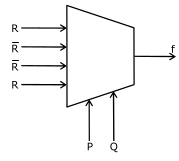
\includegraphics[width=0.2\linewidth]{figs/screenshot001}
			\caption{}
			\label{fig:screenshot001}
		\end{figure}
		

		
		\hfill{\brak{\text{GATE CS 2010}}}
		
		\begin{enumerate}
			\begin{multicols}{4}
				\item $P \oplus Q \oplus R$
				\item $\overline{P \oplus Q \oplus R}$
				\item $P + Q + R$
				\item $\overline{P + Q + R}$
			\end{multicols}
		\end{enumerate}
		
		\item In a binary tree with $n$ nodes, every node has an odd number of descendants. Every node is considered to be its own descendant. What is the number of nodes in the tree that have exactly one child?
		
		\hfill{\brak{\text{GATE CS 2010}}}
		
		\begin{enumerate}
			\begin{multicols}{4}
				\item $0$
				\item $1$
				\item $\brak{n-1}/2$
				\item $n-1$
			\end{multicols}
		\end{enumerate}
		
		\item What does the following program print?
		\begin{verbatim}
			#include <stdio.h>
			void f(int *p, int *q) {
				p = q;
				*p = 2;
			}
			int i = 0, j = 1;
			int main() {
				f(&i, &j);
				printf("%d %d\n", i, j);
				return 0;
			}
		\end{verbatim}
		
		\hfill{\brak{\text{GATE CS 2010}}}
		
		\begin{enumerate}
			\begin{multicols}{4}
				\item $2$ $2$
				\item $2$ $1$
				\item $0$ $1$
				\item $0$ $2$
			\end{multicols}
		\end{enumerate}
		
		\item Two alternative packages $A$ and $B$ are available for processing a database having $10^k$ records. Package $A$ requires $0.0001n^2$ time units and package $B$ requires $10n\log_{10}n$ time units to process $n$ records. What is the smallest value of $k$ for which package $B$ will be preferred over $A$?
		
		\hfill{\brak{\text{GATE CS 2010}}}
		
		\begin{enumerate}
			\begin{multicols}{4}
				\item $12$
				\item $10$
				\item $6$
				\item $5$
			\end{multicols}
		\end{enumerate}
		
		\item Which data structure in a compiler is used for managing information about variables and their attributes?
		
		\hfill{\brak{\text{GATE CS 2010}}}
		
		\begin{enumerate}
			\begin{multicols}{2}
				\item Abstract syntax tree
				\item Symbol table
				\item Semantic stack
				\item Parse table
			\end{multicols}
		\end{enumerate}
		
		\item Which languages necessarily need heap allocation in the runtime environment?
		
		\hfill{\brak{\text{GATE CS 2010}}}
		
		\begin{enumerate}
			\item Those that support recursion
			\item Those that use dynamic scoping
			\item Those that allow dynamic data structures
			\item Those that use global variables
		\end{enumerate}
		
		\item One of the header fields in an IP datagram is the Time to Live $\brak{\text{TTL}}$ field. Which of the following statements best explains the need for this field?
		
		\hfill{\brak{\text{GATE CS 2010}}}
		
		\begin{enumerate}
			\item It can be used to prioritize packets
			\item It can be used to reduce delays
			\item It can be used to optimize throughput
			\item It can be used to prevent packet looping
		\end{enumerate}
		
		\item Which one of the following is not a client server application?
		
		\hfill{\brak{\text{GATE CS 2010}}}
		
		\begin{enumerate}
			\begin{multicols}{4}
				\item Internet chat
				\item Web browsing
				\item E-mail
				\item Ping
			\end{multicols}
		\end{enumerate}
		
		\item Let $L_1$ be a recursive language. Let $L_2$ and $L_3$ be languages that are recursively enumerable but not recursive. Which of the following statements is not necessarily true?
		
		\hfill{\brak{\text{GATE CS 2010}}}
		
		\begin{enumerate}
			\begin{multicols}{2}

	
			\item $L_2 - L_1$ is recursively enumerable
			\item $L_1 - L_3$ is recursively enumerable
			\item $L_2 \cap L_1$ is recursively enumerable
			\item $L_2 \cup L_1$ is recursively enumerable
					\end{multicols}
		\end{enumerate}
		
		\item Consider a $B^+$-tree in which the maximum number of keys in a node is $5$. What is the minimum number of keys in any non-root node?
		
		\hfill{\brak{\text{GATE CS 2010}}}
		
		\begin{enumerate}
			\begin{multicols}{4}
				\item $1$
				\item $2$
				\item $3$
				\item $4$
			\end{multicols}
		\end{enumerate}
		
		\item A relational schema for a train reservation database is given below
		
		Passenger$\brak{\text{pid, pname, age}}$
		
		Reservation$\brak{\text{pid, class, tid}}$
		
		\begin{table}[h]
			\centering
			\caption*{}
			\label{tab:passenger}
			\begin{tabular}{|c|c|c|}
				\hline
				pid & pname & Age \\
				\hline
				0 & 'Sachin' & 65 \\
				1 & 'Rahul' & 66 \\
				2 & 'Sourav' & 67 \\
				3 & 'Anil' & 69 \\
				\hline
			\end{tabular}
		\end{table}
		
		\begin{table}[h]
			\centering
			\caption*{}
			\label{tab:reservation}
			\begin{tabular}{|c|c|c|}
				\hline
				pid & class & tid \\
				\hline
				0 & 'AC' & 8200 \\
				1 & 'AC' & 8201 \\
				2 & 'SC' & 8201 \\
				5 & 'AC' & 8203 \\
				1 & 'SC' & 8204 \\
				3 & 'AC' & 8202 \\
				\hline
			\end{tabular}
		\end{table}
		
		What pids are returned by the following SQL query for the above instance of the tables?
		
		\begin{verbatim}
			SELECT pid
			FROM Reservation
			WHERE class = 'AC' AND
			EXISTS (SELECT *
			FROM Passenger
			WHERE age > 65 AND
			Passenger.pid = Reservation.pid)
		\end{verbatim}
		
		\hfill{\brak{\text{GATE CS 2010}}}
		
		\begin{enumerate}
			\begin{multicols}{4}
				\item $1, 0$
				\item $1, 2$
				\item $1, 3$
				\item $1, 5$
			\end{multicols}
		\end{enumerate}
		
		\item Which of the following concurrency control protocols ensure both conflict serializability and freedom from deadlock?
		
		I. $2$-phase locking
		
		II. Time-stamp ordering
		
		\hfill{\brak{\text{GATE CS 2010}}}
		
		\begin{enumerate}
			\begin{multicols}{4}
				\item I only
				\item II only
				\item Both I and II
				\item Neither I nor II
			\end{multicols}
		\end{enumerate}
		
		\item The cyclomatic complexity of each of the modules $A$ and $B$ shown below is $10$. What is the cyclomatic complexity of the sequential integration shown on the right hand side?
		% Image: q21
		
		\hfill{\brak{\text{GATE CS 2010}}}
		
		\begin{enumerate}
			\begin{multicols}{4}
				\item $19$
				\item $21$
				\item $20$
				\item $10$
			\end{multicols}
		\end{enumerate}
		
		\item What is the appropriate pairing of items in the two columns listing various activities encountered in a software life cycle?
		
		\begin{tabular}{ll}
			P. Requirements Capture & 1. Module Development and Integration \\
			Q. Design & 2. Domain Analysis \\
			R. Implementation & 3. Structural and Behavioral Modeling \\
			S. Maintenance & 4. Performance Tuning \\
		\end{tabular}
		
		\hfill{\brak{\text{GATE CS 2010}}}
		
		\begin{enumerate}
			\begin{multicols}{2}
				\item P-3, Q-2, R-4, S-1
				\item P-2, Q-3, R-1, S-4
				\item P-3, Q-2, R-1, S-4
				\item P-2, Q-3, R-4, S-1
			\end{multicols}
		\end{enumerate}
		
		\item Consider the methods used by processes $P1$ and $P2$ for accessing their critical sections whenever needed, as given below. The initial values of shared boolean variables $S1$ and $S2$ are randomly assigned.
		
		\begin{tabular}{|l|l|}
			\hline
			\textbf{Method used by P1} & \textbf{Method used by P2} \\
			\hline
			while $\brak{S1 == S2}$; & while $\brak{S1 != S2}$; \\
			Critical Section & Critical Section \\
			$S1 = S2$; & $S2 = \text{not}\brak{S1}$; \\
			\hline
		\end{tabular}
		
		Which one of the following statements describes the properties achieved?
		
		\hfill{\brak{\text{GATE CS 2010}}}
		
		\begin{enumerate}
			\begin{multicols}{2}


			\item Mutual exclusion but not progress
			\item Progress but not mutual exclusion
			\item Neither mutual exclusion nor progress
			\item Both mutual exclusion and progress
						\end{multicols}
		\end{enumerate}
		
		\item A system uses FIFO policy for page replacement. It has $4$ page frames with no pages loaded to begin with. The system first accesses $100$ distinct pages in some order and then accesses the same $100$ pages but now in the reverse order. How many page faults will occur?
		
		\hfill{\brak{\text{GATE CS 2010}}}
		
		\begin{enumerate}
			\begin{multicols}{4}
				\item $196$
				\item $192$
				\item $197$
				\item $195$
			\end{multicols}
		\end{enumerate}
		
		\item Which of the following statements are true?
		
		I. Shortest remaining time first scheduling may cause starvation
		
		II. Preemptive scheduling may cause starvation
		
		III. Round robin is better than FCFS in terms of response time
		
		\hfill{\brak{\text{GATE CS 2010}}}
		
		\begin{enumerate}
			\begin{multicols}{4}
				\item I only
				\item I and III only
				\item II and III only
				\item I, II and III
			\end{multicols}
		\end{enumerate}
			\fbox{{\large Q.26 - Q.55 Carry ONE mark each}}\\
		\item Consider a company that assembles computers. The probability of a faulty assembly of any computer is $p$. The company therefore subjects each computer to a testing process. This testing process gives the correct result for any computer with a probability of $q$. What is the probability of a computer being declared faulty?
		
		\hfill{\brak{\text{GATE CS 2010}}}
		
		\begin{enumerate}
			\begin{multicols}{2}
				\item $pq + \brak{1-p}\brak{1-q}$
				\item $\brak{1-q}p$
				\item $\brak{1-p}q$
				\item $pq$
			\end{multicols}
		\end{enumerate}
		
		\item What is the probability that divisor of $10^{99}$ is a multiple of $10^{96}$?
		
		\hfill{\brak{\text{GATE CS 2010}}}
		
		\begin{enumerate}
			\begin{multicols}{4}
				\item $1/625$
				\item $4/625$
				\item $12/625$
				\item $16/625$
			\end{multicols}
		\end{enumerate}
		
		\item The degree sequence of a simple graph is the sequence of the degrees of the nodes in the graph in decreasing order. Which of the following sequences can not be the degree sequence of any graph?
		
		I. $7, 6, 5, 4, 4, 3, 2, 1$
		
		II. $6, 6, 6, 6, 3, 3, 2, 2$
		
		III. $7, 6, 6, 4, 4, 3, 2, 2$
		
		IV. $8, 7, 7, 6, 4, 2, 1, 1$
		
		\hfill{\brak{\text{GATE CS 2010}}}
		
		\begin{enumerate}
			\begin{multicols}{4}
				\item I and II
				\item III and IV
				\item IV only
				\item II and IV
			\end{multicols}
		\end{enumerate}
		
		\item Consider the following matrix
		\begin{align*}
			A = \myvec{2 & 3 \\ x & y}
		\end{align*}
		If the eigenvalues of $A$ are $4$ and $8$, then
		
		\hfill{\brak{\text{GATE CS 2010}}}
		
		\begin{enumerate}
			\begin{multicols}{2}
				\item $x = 4, y = 10$
				\item $x = 5, y = 8$
				\item $x = -3, y = 9$
				\item $x = -4, y = 10$
			\end{multicols}
		\end{enumerate}
		
		\item Suppose the predicate $F\brak{x, y, t}$ is used to represent the statement that person $x$ can fool person $y$ at time $t$. Which one of the statements below expresses best the meaning of the formula $\forall x \exists y \exists t \brak{\neg F\brak{x, y, t}}$?
		
		\hfill{\brak{\text{GATE CS 2010}}}
		
		\begin{enumerate}
			\item Everyone can fool some person at some time
			\item No one can fool everyone all the time
			\item Everyone cannot fool some person all the time
			\item No one can fool some person at some time
		\end{enumerate}
		
		\item What is the Boolean expression for the output $f$ of the combinational logic circuit of NOR gates given below?
\begin{figure}[H]
	\centering
	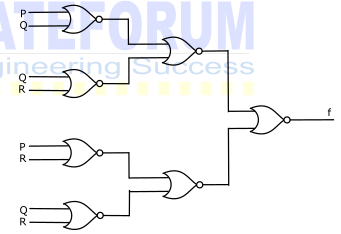
\includegraphics[width=0.3\linewidth]{figs/screenshot002}
	\caption{}
	\label{fig:screenshot002}
\end{figure}

		
		\hfill{\brak{\text{GATE CS 2010}}}
		
		\begin{enumerate}
			\begin{multicols}{4}
				\item $\overline{Q + R}$
				\item $\overline{P + Q}$
				\item $\overline{P + R}$
				\item $\overline{P + Q + R}$
			\end{multicols}
		\end{enumerate}
		
		\item In the sequential circuit shown below, if the initial value of the output $Q_1Q_0$ is $00$, what are the next four values of $Q_1Q_0$?
\begin{figure}[H]
	\centering
	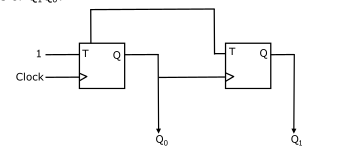
\includegraphics[width=0.3\linewidth]{figs/screenshot003}
	\caption{}
	\label{fig:screenshot003}
\end{figure}

		
		\hfill{\brak{\text{GATE CS 2010}}}
		
		\begin{enumerate}
			\begin{multicols}{4}
				\item $11, 10, 01, 00$
				\item $10, 11, 01, 00$
				\item $10, 00, 01, 11$
				\item $11, 10, 00, 01$
			\end{multicols}
		\end{enumerate}
		
		\item A $5$-stage pipelined processor has Instruction Fetch $\brak{\text{IF}}$, Instruction Decode $\brak{\text{ID}}$, Operand Fetch $\brak{\text{OF}}$, Perform Operation $\brak{\text{PO}}$ and Write Operand $\brak{\text{WO}}$ stages. The IF, ID, OF and WO stages take $1$ clock cycle each for any instruction. The PO stage takes $1$ clock cycle for ADD and SUB instructions, $3$ clock cycles for MUL instruction, and $6$ clock cycles for DIV instruction respectively. Operand forwarding is used in the pipeline. What is the number of clock cycles needed to execute the following sequence of instructions?
		
		\begin{align*}
			&I_0\colon \text{MUL } R_2, R_0, R_1 \quad R_2 \leftarrow R_0 * R_1\\
			&I_1\colon \text{DIV } R_5, R_3, R_4 \quad R_5 \leftarrow R_3 / R_4\\
			&I_2\colon \text{ADD } R_2, R_5, R_2 \quad R_2 \leftarrow R_5 + R_2\\
			&I_3\colon \text{SUB } R_5, R_2, R_6 \quad R_5 \leftarrow R_2 - R_6
		\end{align*}
		
		\hfill{\brak{\text{GATE CS 2010}}}
		
		\begin{enumerate}
			\begin{multicols}{4}
				\item $13$
				\item $15$
				\item $17$
				\item $19$
			\end{multicols}
		\end{enumerate}
		
		\item The weight of a sequence $a_0, a_1, \ldots, a_{n-1}$ of real numbers is defined as $a_0 + a_1/2 + \ldots + a_{n-1}/2^{n-1}$. A subsequence of a sequence is obtained by deleting some elements from the sequence, keeping the order of the remaining elements the same. Let $X$ denote the maximum possible weight of a subsequence of $a_0, a_1, \ldots, a_{n-1}$. Then $X$ is equal to
		
		\hfill{\brak{\text{GATE CS 2010}}}
		
		\begin{enumerate}
			\begin{multicols}{4}
				\item $\max\brak{Y, a_0 + Y}$
				\item $\max\brak{Y, a_0 + Y/2}$
				\item $\max\brak{Y, a_0 + 2Y}$
				\item $a_0 + Y/2$
			\end{multicols}
		\end{enumerate}
		
		\item What is the value printed by the following C program?
		\begin{verbatim}
			#include <stdio.h>
			int f(int *a, int n)
			{
				if (n <= 0) return 0;
				else if (*a % 2 == 0) return *a + f(a+1, n-1);
				else return *a - f(a+1, n-1);
			}
			int main()
			{
				int a[] = {12, 7, 13, 4, 11, 6};
				printf("%d", f(a, 6));
				return 0;
			}
		\end{verbatim}
		
		\hfill{\brak{\text{GATE CS 2010}}}
		
		\begin{enumerate}
			\begin{multicols}{4}
				\item $-9$
				\item $5$
				\item $15$
				\item $19$
			\end{multicols}
		\end{enumerate}
		
		\item The following C function takes a simply-linked list as input argument. It modifies the list by moving the last element to the front of the list and returns the modified list. Some part of the code is left blank.
		
		\begin{verbatim}
			typedef struct node {
				int value;
				struct node *next;
			} Node;
			
			Node *move_to_front(Node *head) {
				Node *p, *q;
				if ((head == NULL) || (head->next == NULL)) return head;
				q = NULL; p = head;
				while (p->next != NULL) {
					q = p;
					p = p->next;
				}
				_______________________________
				return head;
			}
		\end{verbatim}
		
		Choose the correct alternative to replace the blank line.
		
		\hfill{\brak{\text{GATE CS 2010}}}
		
		\begin{enumerate}
			\item q = NULL; p->next = head; head = p;
			\item q->next = NULL; head = p; p->next = head;
			\item head = p; p->next = q; q->next = NULL;
			\item q->next = NULL; p->next = head; head = p;
		\end{enumerate}
		
		\item The program below uses six temporary variables a, b, c, d, e, f.
		\begin{verbatim}
			a = 1
			b = 10
			c = 20
			d = a + b
			e = c + d
			f = c + e
			b = c + e
			e = b + f
			d = 5 + e
			return d + f
		\end{verbatim}
		
		Assuming that all operations take their operands from registers, what is the minimum number of registers needed to execute this program without spilling?
		
		\hfill{\brak{\text{GATE CS 2010}}}
		
		\begin{enumerate}
			\begin{multicols}{4}
				\item $2$
				\item $3$
				\item $4$
				\item $6$
			\end{multicols}
		\end{enumerate}
		
		\item The grammar $S \to aSa \mid bS \mid c$ is
		
		\hfill{\brak{\text{GATE CS 2010}}}
		
		\begin{enumerate}
			\begin{multicols}{2}
				\item LL$\brak{1}$ but not LR$\brak{1}$
				\item LR$\brak{1}$ but not LL$\brak{1}$
				\item Both LL$\brak{1}$ and LR$\brak{1}$
				\item Neither LL$\brak{1}$ nor LR$\brak{1}$
			\end{multicols}
		\end{enumerate}
		
		\item Let $L = \{w \in \brak{0+1}^* \mid w \text{ has even number of 1s}\}$, i.e. $L$ is the set of all bit strings with even number of $1$s. Which one of the regular expressions below represents $L$?
		
		\hfill{\brak{\text{GATE CS 2010}}}
		
		\begin{enumerate}
			\begin{multicols}{4}
				\item $\brak{0^*10^*1}^*$
				\item $0^*\brak{10^*10^*}^*$
				\item $0^*\brak{10^*1}^*0^*$
				\item $0^*1\brak{10^*1}^*10^*$
			\end{multicols}
		\end{enumerate}
		
		\item Consider the languages $L_1 = \{0^i1^j \mid i \neq j\}$, $L_2 = \{0^i1^j \mid i = j\}$, $L_3 = \{0^i1^j \mid i = 2j+1\}$, $L_4 = \{0^i1^j \mid i \neq 2j\}$. Which one of the following statements is true?
		
		\hfill{\brak{\text{GATE CS 2010}}}
		
		\begin{enumerate}
			\begin{multicols}{2}


			\item Only $L_2$ is context free
			\item Only $L_2$ and $L_3$ are context free
			\item Only $L_1$ and $L_2$ are context free
			\item All are context 
						\end{multicols}
		\end{enumerate}
		
		\item Let $w$ be any string of length $n$ in $\{0, 1\}^*$. Let $L$ be the set of all substrings of $w$. What is the minimum number of states in a non-deterministic finite automaton that accepts $L$?
		
		\hfill{\brak{\text{GATE CS 2010}}}
		
		\begin{enumerate}
			\begin{multicols}{4}
				\item $n-1$
				\item $n$
				\item $n+1$
				\item $2^{n-1}$
			\end{multicols}
		\end{enumerate}
		
		\item Consider the following schedule for transactions $T_1$, $T_2$ and $T_3$:
		
		\begin{table}[h]
			\centering
			\caption*{}
			\label{tab:schedule}
			\begin{tabular}{|c|c|c|}
				\hline
				$T_1$ & $T_2$ & $T_3$ \\
				\hline
				Read$\brak{X}$ & & \\
				& Read$\brak{Y}$ & \\
				& & Read$\brak{Y}$ \\
				& Write$\brak{Y}$ & \\
				& & Write$\brak{X}$ \\
				& Write$\brak{X}$ & \\
				Read$\brak{X}$ & & \\
				Write$\brak{X}$ & & \\
				\hline
			\end{tabular}
		\end{table}
		
		Which one of the schedules below is the correct serialization of the above?
		
		\hfill{\brak{\text{GATE CS 2010}}}
		
		\begin{enumerate}
			\begin{multicols}{2}
				\item $T_1 \to T_3 \to T_2$
				\item $T_2 \to T_1 \to T_3$
				\item $T_2 \to T_3 \to T_1$
				\item $T_3 \to T_1 \to T_2$
			\end{multicols}
		\end{enumerate}
		
		\item The following functional dependencies hold for relations $R\brak{A, B, C}$ and $S\brak{B, D, E}$:
		\begin{align*}
			B &\to A\\
			A &\to C
		\end{align*}
		The relation $R$ contains $200$ tuples and the relation $S$ contains $100$ tuples. What is the maximum number of tuples possible in the natural join $R \bowtie S$?
		
		\hfill{\brak{\text{GATE CS 2010}}}
		
		\begin{enumerate}
			\begin{multicols}{4}
				\item $100$
				\item $200$
				\item $300$
				\item $2000$
			\end{multicols}
		\end{enumerate}
		
		\item The following program is to be tested for statement coverage:
		\begin{verbatim}
			begin
			if (a == b) {S1; exit;}
			else if (c == d) {S2;}
			else {S3; exit;}
			S4;
			end
		\end{verbatim}
		
		The test cases $T_1$, $T_2$, $T_3$ and $T_4$ given below are expressed in terms of the properties satisfied by the values of variables $a$, $b$, $c$ and $d$. The exact values are not given.
		
		$T_1$: $a$, $b$, $c$ and $d$ are all equal
		
		$T_2$: $a$, $b$, $c$ and $d$ are all distinct
		
		$T_3$: $a = b$ and $c \neq d$
		
		$T_4$: $a \neq b$ and $c = d$
		
		Which of the test suites given below ensures coverage of statements $S_1$, $S_2$, $S_3$ and $S_4$?
		
		\hfill{\brak{\text{GATE CS 2010}}}
		
		\begin{enumerate}
			\begin{multicols}{4}
				\item $T_1, T_2, T_3$
				\item $T_2, T_4$
				\item $T_3, T_4$
				\item $T_1, T_2, T_4$
			\end{multicols}
		\end{enumerate}
		
		\item The following program consists of $3$ concurrent processes and $3$ binary semaphores. The semaphores are initialized as $S_0 = 1$, $S_1 = 0$, $S_2 = 0$.
		
		\begin{table}[h]
			\centering
			\caption*{}
			\label{tab:processes}
			\begin{tabular}{|l|l|l|}
				\hline
				Process P0 & Process P1 & Process P2 \\
				\hline
				while $\brak{\text{true}}$ \{ & wait $\brak{S_1}$; & wait $\brak{S_2}$; \\
				\quad wait $\brak{S_0}$; & Release $\brak{S_0}$; & release $\brak{S_0}$; \\
				\quad print '0' & & \\
				\quad release $\brak{S_1}$; & & \\
				\quad release $\brak{S_2}$; & & \\
				\} & & \\
				\hline
			\end{tabular}
		\end{table}
		
		How many times will process $P_0$ print '$0$'?
		
		\hfill{\brak{\text{GATE CS 2010}}}
		
		\begin{enumerate}
			\begin{multicols}{4}
				\item At least twice
				\item Exactly twice
				\item Exactly thrice
				\item Exactly once
			\end{multicols}
		\end{enumerate}
		
		\item A system has $n$ resources $R_0, \ldots, R_{n-1}$, and $k$ processes $P_0, \ldots, P_{k-1}$. The implementation of the resource request logic of each process $P_i$ is as follows:
		
		\begin{verbatim}
			if (i % 2 == 0) {
				if (i < n) request R_i;
				if (i+2 < n) request R_{i+2};
			}
			else {
				if (i < n) request R_{n-i};
				if (i+2 < n) request R_{n-i-2};
			}
		\end{verbatim}
		
		In which one of the following situations is a deadlock possible?
		
		\hfill{\brak{\text{GATE CS 2010}}}
		
		\begin{enumerate}
			\begin{multicols}{4}
				\item $n = 40, k = 26$
				\item $n = 21, k = 12$
				\item $n = 20, k = 10$
				\item $n = 41, k = 19$
			\end{multicols}
		\end{enumerate}
		
		\item Suppose computers $A$ and $B$ have IP addresses $10.105.1.113$ and $10.105.1.91$ respectively and they both use the same net mask $N$. Which of the values of $N$ given below should not be used if $A$ and $B$ should belong to the same network?
		
		\hfill{\brak{\text{GATE CS 2010}}}
		
		\begin{enumerate}
			\begin{multicols}{2}
				\item $255.255.255.0$
				\item $255.255.255.128$
				\item $255.255.255.192$
				\item $255.255.255.224$
			\end{multicols}
		\end{enumerate}
		
		\centering{\textbf{\large Common Data Questions: 48 and 49}}\\
		\item A computer system has an L1 cache, an L2 cache, and a main memory unit connected as shown below. The block size in L1 cache is $4$ words. The block size in L2 cache is $16$ words. The memory access times are $2$ nanoseconds, $20$ nanoseconds and $200$ nanoseconds for L1 cache, L2 cache and main memory unit respectively.
\begin{figure}[H]
	\centering
	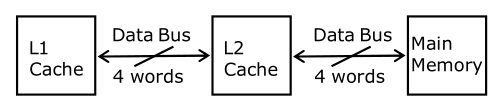
\includegraphics[width=0.38\linewidth]{figs/screenshot004}
	\caption{}
	\label{fig:screenshot004}
\end{figure}

		
		When there is a miss in L1 cache and a hit in L2 cache, a block is transferred from L2 cache to L1 cache. What is the time taken for this transfer?
		
		\hfill{\brak{\text{GATE CS 2010}}}
		
		\begin{enumerate}
			\begin{multicols}{4}
				\item $2$ nanoseconds
				\item $20$ nanoseconds
				\item $22$ nanoseconds
				\item $88$ nanoseconds
			\end{multicols}
		\end{enumerate}
		
		\item When there is a miss in both L1 cache and L2 cache, first a block is transferred from main memory to L2 cache, and then a block is transferred from L2 cache to L1 cache. What is the total time taken for these transfers?
		
		\hfill{\brak{\text{GATE CS 2010}}}
		
		\begin{enumerate}
			\begin{multicols}{4}
				\item $222$ nanoseconds
				\item $888$ nanoseconds
				\item $902$ nanoseconds
				\item $968$ nanoseconds
			\end{multicols}
		\end{enumerate}
				\textbf{\large Common Data Questions: 50 and 51}\\
		 Consider a complete undirected graph with vertex set $\{0, 1, 2, 3, 4\}$. Entry $W_{ij}$ in the matrix $W$ below is the weight of the edge $\{i, j\}$.
		
		\begin{align*}
			W = \myvec{
				0 & 1 & 8 & 1 & 4 \\
				1 & 0 & 12 & 4 & 9 \\
				8 & 12 & 0 & 7 & 3 \\
				1 & 4 & 7 & 0 & 2 \\
				4 & 9 & 3 & 2 & 0
			}
		\end{align*}
		
		\item What is the minimum possible weight of a spanning tree $T$ in this graph such that vertex $0$ is a leaf node in the tree $T$?
		
		\hfill{\brak{\text{GATE CS 2010}}}
		
		\begin{enumerate}
			\begin{multicols}{4}
				\item $7$
				\item $8$
				\item $9$
				\item $10$
			\end{multicols}
		\end{enumerate}
		
		\item What is the minimum possible weight of a path $P$ from vertex $1$ to vertex $2$ in this graph such that $P$ contains at most $3$ edges?
		
		\hfill{\brak{\text{GATE CS 2010}}}
		
		\begin{enumerate}
			\begin{multicols}{4}
				\item $7$
				\item $8$
				\item $9$
				\item $10$
			\end{multicols}
		\end{enumerate}
	\textbf{\large Linked Answer Questions: Q.52 to Q.55 Carry Two Marks Each\\
							Statement for Linked Answer Questions: 52 and 53}\\
A hash table of length $10$ uses open addressing with hash function $h\brak{k} = k \bmod 10$, and linear probing. After inserting $6$ values into an empty hash table, the table is as shown below
		
		\begin{table}[h]
			\centering
			\caption*{}
			\label{tab:hashtable}
			\begin{tabular}{|c|c|}
				\hline
				0 & \\
				\hline
				1 & \\
				\hline
				2 & 42 \\
				\hline
				3 & 23 \\
				\hline
				4 & 34 \\
				\hline
				5 & 52 \\
				\hline
				6 & 46 \\
				\hline
				7 & 33 \\
				\hline
				8 & \\
				\hline
				9 & \\
				\hline
			\end{tabular}
		\end{table}
		
		
		\item Which one of the following choices gives a possible order in which the key values could have been inserted in the table?
		
		\hfill{\brak{\text{GATE CS 2010}}}
		
		\begin{enumerate}
			\begin{multicols}{2}
				\item $46, 42, 34, 52, 23, 33$
				\item $34, 42, 23, 52, 33, 46$
				\item $46, 34, 42, 23, 52, 33$
				\item $42, 46, 33, 23, 34, 52$
			\end{multicols}
		\end{enumerate}
		
		\item How many different insertion sequences of the key values using the same hash function and linear probing will result in the hash table shown above?
		
		\hfill{\brak{\text{GATE CS 2010}}}
		
		\begin{enumerate}
			\begin{multicols}{4}
				\item $10$
				\item $20$
				\item $30$
				\item $40$
			\end{multicols}
		\end{enumerate}

				\textbf{\large Statement for Linked Answer Questions: 54 and 55}\\
Consider a network with $6$ routers $R_1$ to $R_6$ connected with links having weights as shown in the following diagram.\\
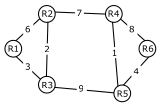
\includegraphics[width=0.5\linewidth]{figs/screenshot005}
\item All the routers use the distance vector based routing algorithm to update their routing tables.Eachrouter starts with its routing table initialized to contain an entry for each neighbour with the weightof the respective connecting link. After all the routing tables stabilize, how many links in the network will never be used for carrying any data?
		\hfill{\brak{\text{GATE CS 2010}}}
		
		\begin{enumerate}
			\begin{multicols}{4}
				\item $4$
				\item $3$
				\item $2$
				\item $1$
			\end{multicols}
		\end{enumerate}
		
		\item Suppose the weights of all unused links in the previous question are changed to $2$ and the distance vector algorithm is used again until all routing tables stabilize. How many links will now remain unused?
		
		\hfill{\brak{\text{GATE CS 2010}}}
		
		\begin{enumerate}
			\begin{multicols}{4}
				\item $0$
				\item $1$
				\item $2$
				\item $3$
			\end{multicols}
		\end{enumerate}
		\textbf{\large Q. No 56 and 60 Carry one mark each}\\
\item Choose the most appropriate word from the options given below to complete the following sentence:\\
His rather casual remarks on politics \underline{\hspace{2cm}} his lack of seriousness about the subject.
		
		\hfill{\brak{\text{GATE CS 2010}}}
		
		\begin{enumerate}
			\begin{multicols}{4}
				\item masked
				\item belied
				\item betrayed
				\item suppressed
			\end{multicols}
		\end{enumerate}
		
		\item Which of the following options is closest in meaning to the word Circuitous.
		\hfill{\brak{\text{GATE CS 2010}}}
		
		\begin{enumerate}
			\begin{multicols}{4}
				\item cyclic
				\item indirect
				\item confusing
				\item crooked
			\end{multicols}
		\end{enumerate}
\item Choose the most appropriate word from the options given below to complete the following sentence:If we manage to \underline{\hspace{2cm}} our natural resources, we would leave a better planet for our children.
\hfill{\brak{\text{GATE CS 2010}}}
		
		\begin{enumerate}
			\begin{multicols}{4}
				\item uphold
				\item restrain
				\item cherish
				\item conserve
			\end{multicols}
		\end{enumerate}
		
		\item $25$ persons are in a room. $15$ of them play hockey, $17$ of them play football and $10$ of them play both hockey and football. Then the number of persons playing neither hockey nor football is:
		\hfill{\brak{\text{GATE CS 2010}}}
		
		\begin{enumerate}
			\begin{multicols}{4}
				\item $2$
				\item $17$
				\item $13$
				\item $3$
			\end{multicols}
		\end{enumerate}
		
		\item The question below consists of a pair of related words followed by four pairs of words. Select the pair that best expresses the relation in the original pair.Unemployed: Worker
		\hfill{\brak{\text{GATE CS 2010}}}
		
		\begin{enumerate}
			\begin{multicols}{4}
				\item fallow: land
				\item unaware: sleeper
				\item wit: jester
				\item renovated: house
			\end{multicols}
		\end{enumerate}
\textbf{\large{Q. No. 61 – 65 Carry Two Marks Each}}
\item If $137 + 276 = 435$, how much is $731 + 672$?
		\hfill{\brak{\text{GATE CS 2010}}}
	
	\begin{multicols}{4}
		\begin{enumerate}
			\item $534$
			\item $1403$
			\item $1623$
			\item $1513$
		\end{enumerate}
	\end{multicols}
	\item Hari $\brak{H}$, Gita $\brak{G}$, Irfan $\brak{I}$ and Saira $\brak{S}$ are siblings $\brak{\text{i.e. brothers and sisters}}$. All were born on $1^{\text{st}}$ January. The age difference between any two successive siblings $\brak{\text{that is born one after another}}$ is less than $3$ years. Given the following facts:\\
i. Hari's age $+$ Gita's age $>$ Irfan's age $+$ Saira's age.\\
ii. The age difference between Gita and Saira is $1$ year. However Gita is not the oldest and Saira is not the youngest.\\
iii. There are no twins.\\
In what order were they born \brak{\text{oldest first}}?
\hfill{\brak{\text{GATE CS 2010}}}
		
		\begin{enumerate}
			\begin{multicols}{4}
				\item HSIG
				\item SGHI
				\item IGSH
				\item IHSG
			\end{multicols}
		\end{enumerate}
		
		\item Modern warfare has changed from large scale clashes of armies to suppression of civilian populations. Chemical agents that do their work silently appear to be suited to such warfare; and regretfully, there exist people in military establishments who think that chemical agents are useful tools for their cause.
		Which of the following statements best sums up the meaning of the above passage:
		\hfill{\brak{\text{GATE CS 2010}}}
		
		\begin{enumerate}
			\item Modern warfare has resulted in civil strife.
			\item Chemical agents are useful in modern warfare.
			\item Use of chemical agents in warfare would be undesirable.
			\item People in military establishments like to use chemical agents in war.
		\end{enumerate}
		
		\item $5$ skilled workers can build a wall in $20$ days; $8$ semi-skilled workers can build a wall in $25$ days; $10$ unskilled workers can build a wall in $30$ days. If a team has $2$ skilled, $6$ semi-skilled and $5$ unskilled workers, how long will it take to build the wall?
		\hfill{\brak{\text{GATE CS 2010}}}
		
		\begin{enumerate}
			\begin{multicols}{4}
				\item $20$
				\item $18$
				\item $16$
				\item $15$
			\end{multicols}
		\end{enumerate}
		
		\item Given digits $2, 2, 3, 3, 4, 4, 4, 4$ how many distinct $4$ digit numbers greater than $3000$ can be formed?
		
		\hfill{\brak{\text{GATE CS 2010}}}
		
		\begin{enumerate}
			\begin{multicols}{4}
				\item $50$
				\item $51$
				\item $52$
				\item $54$
			\end{multicols}
		\end{enumerate}
		
	\end{enumerate}
\end{document}